\documentclass[]{article}
\usepackage{lmodern}
\usepackage{amssymb,amsmath}
\usepackage{ifxetex,ifluatex}
\usepackage{fixltx2e} % provides \textsubscript
\ifnum 0\ifxetex 1\fi\ifluatex 1\fi=0 % if pdftex
  \usepackage[T1]{fontenc}
  \usepackage[utf8]{inputenc}
\else % if luatex or xelatex
  \ifxetex
    \usepackage{mathspec}
  \else
    \usepackage{fontspec}
  \fi
  \defaultfontfeatures{Ligatures=TeX,Scale=MatchLowercase}
\fi
% use upquote if available, for straight quotes in verbatim environments
\IfFileExists{upquote.sty}{\usepackage{upquote}}{}
% use microtype if available
\IfFileExists{microtype.sty}{%
\usepackage{microtype}
\UseMicrotypeSet[protrusion]{basicmath} % disable protrusion for tt fonts
}{}
\usepackage[margin=1in]{geometry}
\usepackage{hyperref}
\hypersetup{unicode=true,
            pdftitle={EAS596, Homework\_4},
            pdfauthor={Abhishek Kumar, Class\#1},
            pdfborder={0 0 0},
            breaklinks=true}
\urlstyle{same}  % don't use monospace font for urls
\usepackage{graphicx,grffile}
\makeatletter
\def\maxwidth{\ifdim\Gin@nat@width>\linewidth\linewidth\else\Gin@nat@width\fi}
\def\maxheight{\ifdim\Gin@nat@height>\textheight\textheight\else\Gin@nat@height\fi}
\makeatother
% Scale images if necessary, so that they will not overflow the page
% margins by default, and it is still possible to overwrite the defaults
% using explicit options in \includegraphics[width, height, ...]{}
\setkeys{Gin}{width=\maxwidth,height=\maxheight,keepaspectratio}
\IfFileExists{parskip.sty}{%
\usepackage{parskip}
}{% else
\setlength{\parindent}{0pt}
\setlength{\parskip}{6pt plus 2pt minus 1pt}
}
\setlength{\emergencystretch}{3em}  % prevent overfull lines
\providecommand{\tightlist}{%
  \setlength{\itemsep}{0pt}\setlength{\parskip}{0pt}}
\setcounter{secnumdepth}{0}
% Redefines (sub)paragraphs to behave more like sections
\ifx\paragraph\undefined\else
\let\oldparagraph\paragraph
\renewcommand{\paragraph}[1]{\oldparagraph{#1}\mbox{}}
\fi
\ifx\subparagraph\undefined\else
\let\oldsubparagraph\subparagraph
\renewcommand{\subparagraph}[1]{\oldsubparagraph{#1}\mbox{}}
\fi

%%% Use protect on footnotes to avoid problems with footnotes in titles
\let\rmarkdownfootnote\footnote%
\def\footnote{\protect\rmarkdownfootnote}

%%% Change title format to be more compact
\usepackage{titling}

% Create subtitle command for use in maketitle
\newcommand{\subtitle}[1]{
  \posttitle{
    \begin{center}\large#1\end{center}
    }
}

\setlength{\droptitle}{-2em}

  \title{EAS596, Homework\_4}
    \pretitle{\vspace{\droptitle}\centering\huge}
  \posttitle{\par}
    \author{Abhishek Kumar, Class\#1}
    \preauthor{\centering\large\emph}
  \postauthor{\par}
      \predate{\centering\large\emph}
  \postdate{\par}
    \date{26/11/2018}


\begin{document}
\maketitle

\subsection{SOLUTION 1}\label{solution-1}

\begin{verbatim}
## 'data.frame':    97 obs. of  10 variables:
##  $ lcavol : num  -0.58 -0.994 -0.511 -1.204 0.751 ...
##  $ lweight: num  2.77 3.32 2.69 3.28 3.43 ...
##  $ age    : int  50 58 74 58 62 50 64 58 47 63 ...
##  $ lbph   : num  -1.39 -1.39 -1.39 -1.39 -1.39 ...
##  $ svi    : int  0 0 0 0 0 0 0 0 0 0 ...
##  $ lcp    : num  -1.39 -1.39 -1.39 -1.39 -1.39 ...
##  $ gleason: int  6 6 7 6 6 6 6 6 6 6 ...
##  $ pgg45  : int  0 0 20 0 0 0 0 0 0 0 ...
##  $ lpsa   : num  -0.431 -0.163 -0.163 -0.163 0.372 ...
##  $ train  : logi  TRUE TRUE TRUE TRUE TRUE TRUE ...
\end{verbatim}

\begin{verbatim}
## Minimum Classification Error while using Cp is at k =  5
\end{verbatim}

\begin{verbatim}
## Minimum Classification Error while using BIC is at k =  3
\end{verbatim}

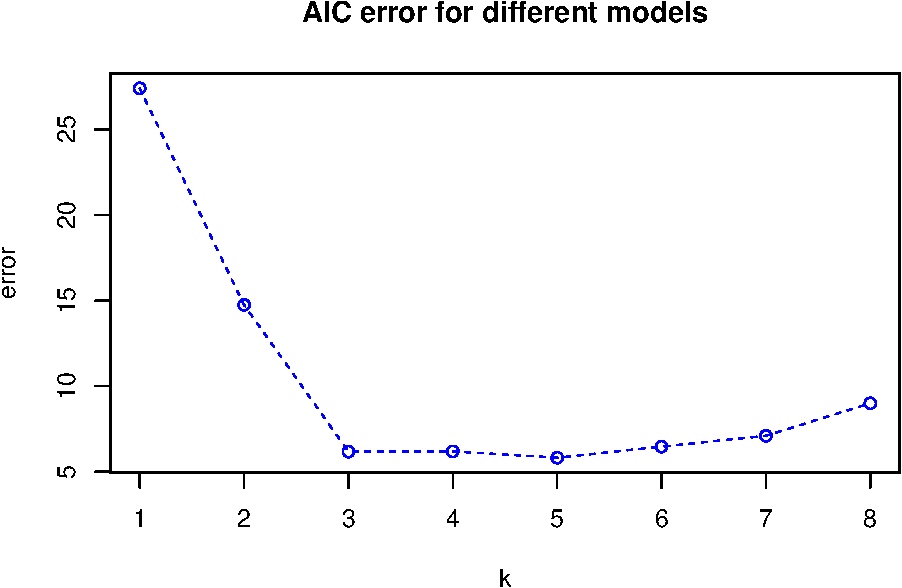
\includegraphics{HW4_Solution_files/figure-latex/unnamed-chunk-1-1.pdf}
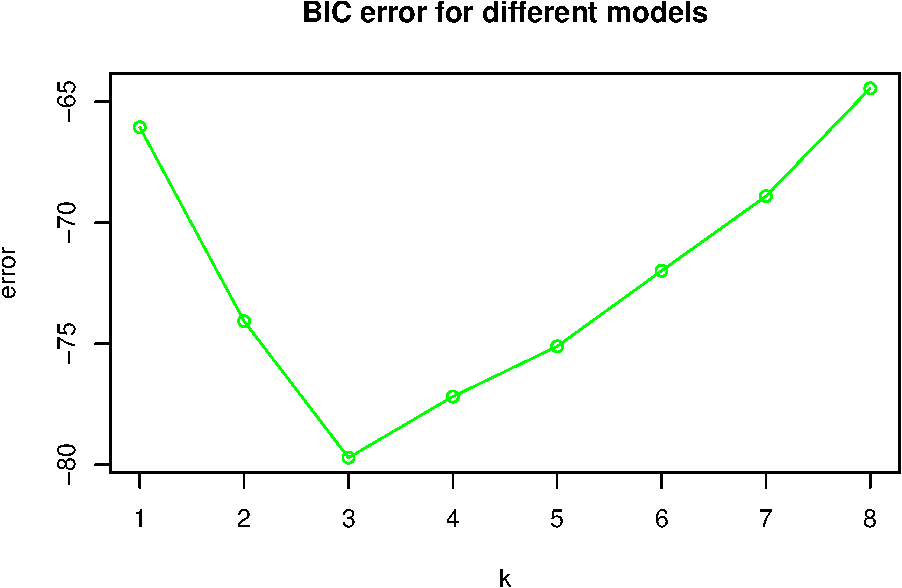
\includegraphics{HW4_Solution_files/figure-latex/unnamed-chunk-1-2.pdf}
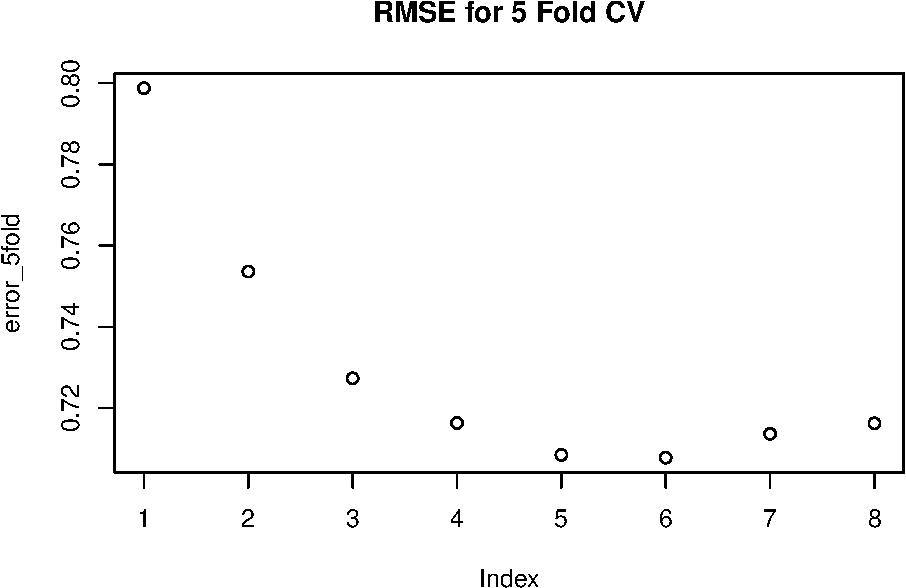
\includegraphics{HW4_Solution_files/figure-latex/unnamed-chunk-2-1.pdf}

\begin{verbatim}
## The minimum error with 5 fold cross-validation is at k =  6
\end{verbatim}

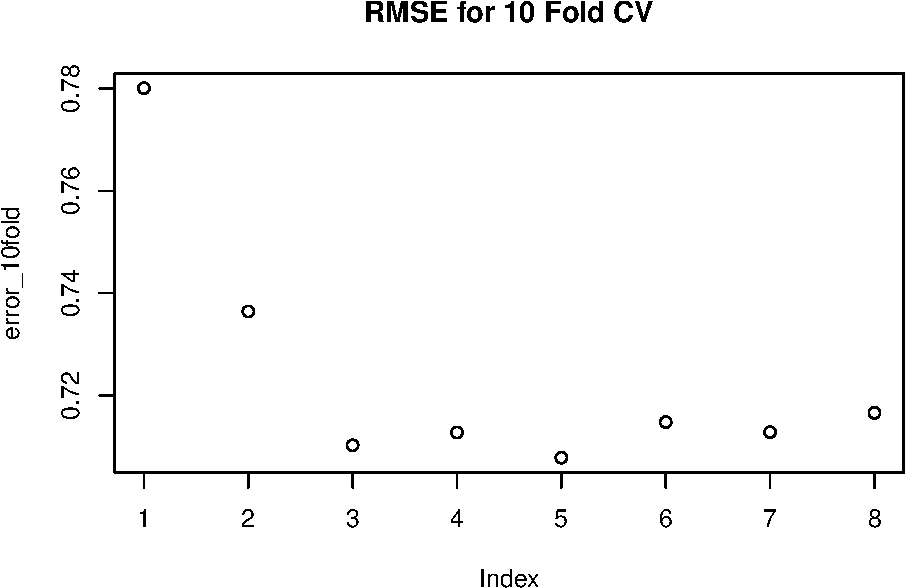
\includegraphics{HW4_Solution_files/figure-latex/unnamed-chunk-2-2.pdf}

\begin{verbatim}
## The minimum error with 10 fold cross-validation is at k =  5
\end{verbatim}

~

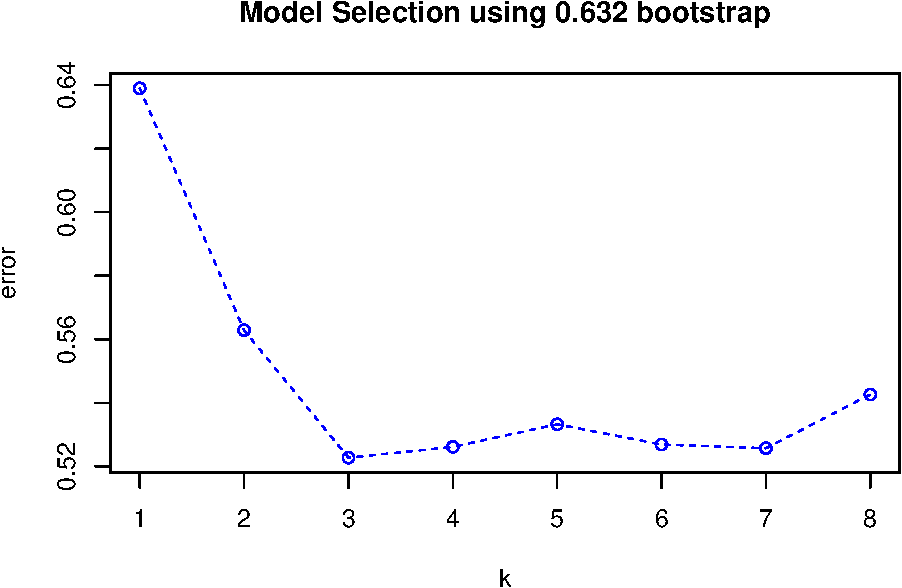
\includegraphics{HW4_Solution_files/figure-latex/unnamed-chunk-3-1.pdf}

\newpage

\begin{verbatim}
##          lcavol lweight age lbph svi lcp gleason pgg45
## 1  ( 1 ) "*"    " "     " " " "  " " " " " "     " "  
## 2  ( 1 ) "*"    "*"     " " " "  " " " " " "     " "  
## 3  ( 1 ) "*"    "*"     " " " "  "*" " " " "     " "  
## 4  ( 1 ) "*"    "*"     " " "*"  "*" " " " "     " "  
## 5  ( 1 ) "*"    "*"     "*" "*"  "*" " " " "     " "  
## 6  ( 1 ) "*"    "*"     "*" "*"  "*" " " " "     "*"  
## 7  ( 1 ) "*"    "*"     "*" "*"  "*" "*" " "     "*"  
## 8  ( 1 ) "*"    "*"     "*" "*"  "*" "*" "*"     "*"
\end{verbatim}

We see that almost all the methods agree that the best model is
approximately at k(number of features in the model) = 3,5,6. We should
select k=3 as it will not overfit the data as we are including less
number of variables in the model.

\subsection{SOLUTION 2}\label{solution-2}

\begin{verbatim}
## Mean Classification Test Error:  0.08333333
\end{verbatim}

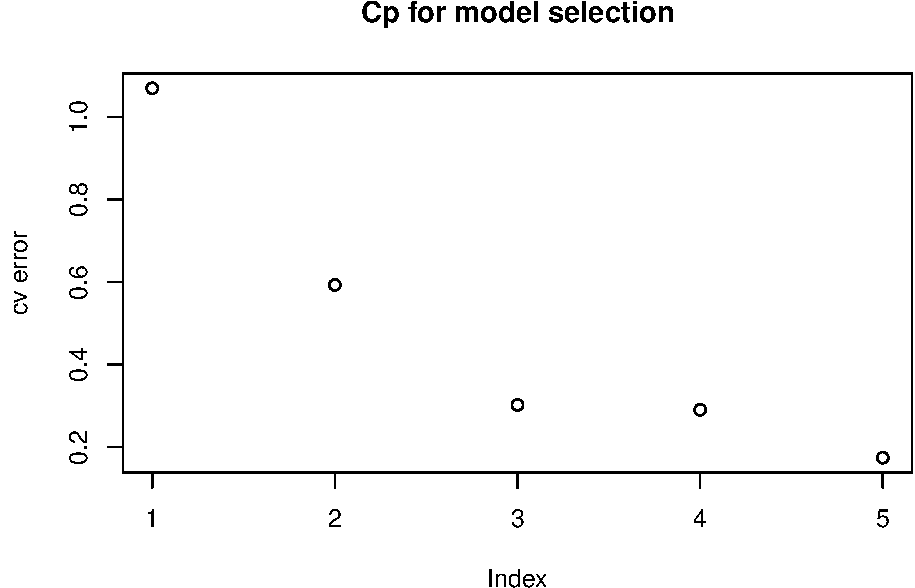
\includegraphics{HW4_Solution_files/figure-latex/unnamed-chunk-5-1.pdf}

~

\begin{center}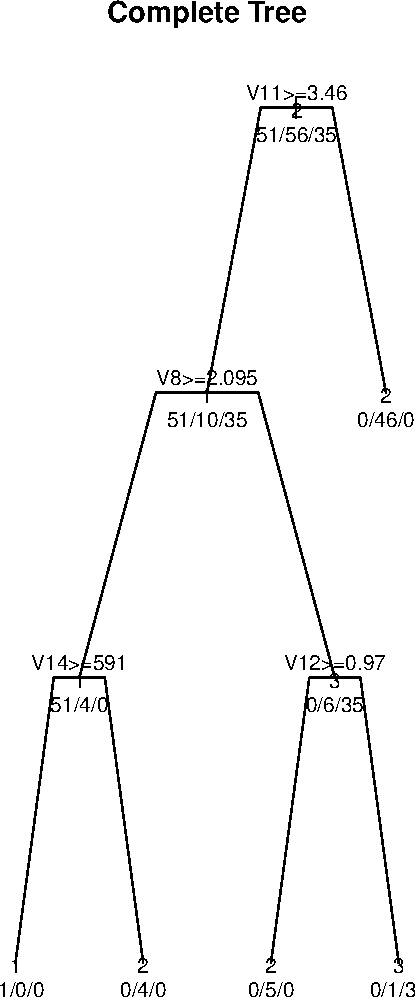
\includegraphics{HW4_Solution_files/figure-latex/unnamed-chunk-6-1} \end{center}

\begin{verbatim}
## Mean Classification Test Error :  0.08333333
\end{verbatim}

~

\newpage

\begin{center}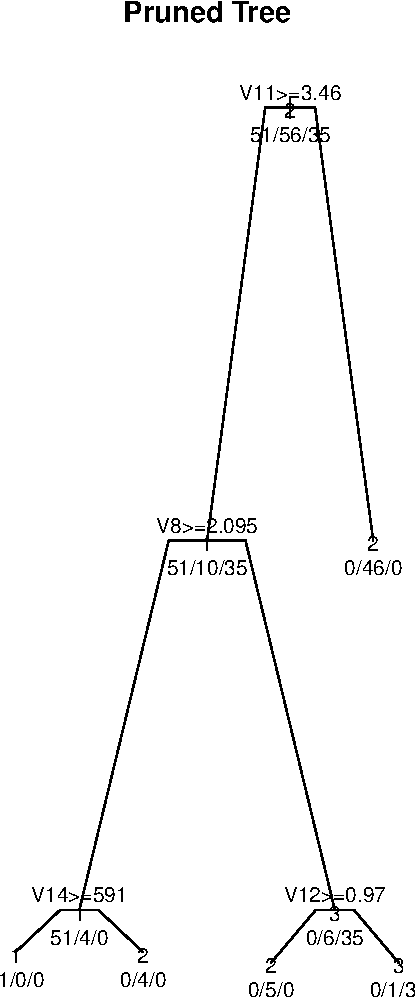
\includegraphics{HW4_Solution_files/figure-latex/unnamed-chunk-7-1} \end{center}

\begin{verbatim}
## Mean Classification Test Error :  0.08333333
\end{verbatim}

~

Calculating number of training and test data falling on each node:

\begin{verbatim}
## No. of training data falling on node 1 is  51
\end{verbatim}

\begin{verbatim}
## No. of test data falling on node 1 is  11
\end{verbatim}

\begin{verbatim}
## No. of training data falling on node 2 is  4
\end{verbatim}

\begin{verbatim}
## No. of test data falling on node 1 is  0
\end{verbatim}

\begin{verbatim}
## No. of training data falling on node 3 is  5
\end{verbatim}

\begin{verbatim}
## No. of test data falling on node 3 is  16
\end{verbatim}

\begin{verbatim}
## No. of training data falling on node 4 is  36
\end{verbatim}

\begin{verbatim}
## No. of test data falling on node 4 is  0
\end{verbatim}

\begin{verbatim}
## No. of training data falling on node 5 is  46
\end{verbatim}

\begin{verbatim}
## No. of test data falling on node 5 is  9
\end{verbatim}

\newpage

The confusion matrix foe the test set is :

\begin{verbatim}
##    tree_pred
##      1  2  3
##   1  8  0  0
##   2  3 12  0
##   3  0  0 13
\end{verbatim}

The tree was built using minimum split of 5, number of cross validations
= 10 and the value of complexity parameter to be = 0 after iterating
through all permutations of these parameters. And then we pruned the
tree with complexity parameter, cp as the minimum error using
cross-validation on the complete tree.

Let's look at the pruned tree and see how many data points fall into
each node(leaves). We have 5 leaves node and as we can see from the tree
plot that 46, 51, 4, 5 and 36 data points falls into each leaf nodes
respectively.

~

\subsection{SOLUTION 3}\label{solution-3}

We will use Boston dataset and try to classify houses that lies in high
crime zone or not. For this we will assume high crime zones where crime
rate is more than the median crime rate and low crime zone where crime
rate is below median crime rate.

\begin{verbatim}
## Logistic Regression Train Error :  0.0817942
\end{verbatim}

\begin{verbatim}
## 
##  Logistic Regression Test error :  0.1102362
\end{verbatim}

\begin{verbatim}
## Loading required package: class
\end{verbatim}

\begin{verbatim}
## KNN Test Error for k=1:10, : 0.1181102 0.08661417 0.1102362 0.07874016 0.09448819 0.07874016 0.09448819 0.1102362 0.1102362
\end{verbatim}

\begin{verbatim}
## For KNN, the test error is minimum at, K= 4  and the test Error is :  0.07874016
\end{verbatim}

\begin{verbatim}
## Classifiaction error for a Single Tree : 0.03937008
\end{verbatim}

\begin{verbatim}
## Classification Error for a Single Tree with pruning:  0.05511811
\end{verbatim}

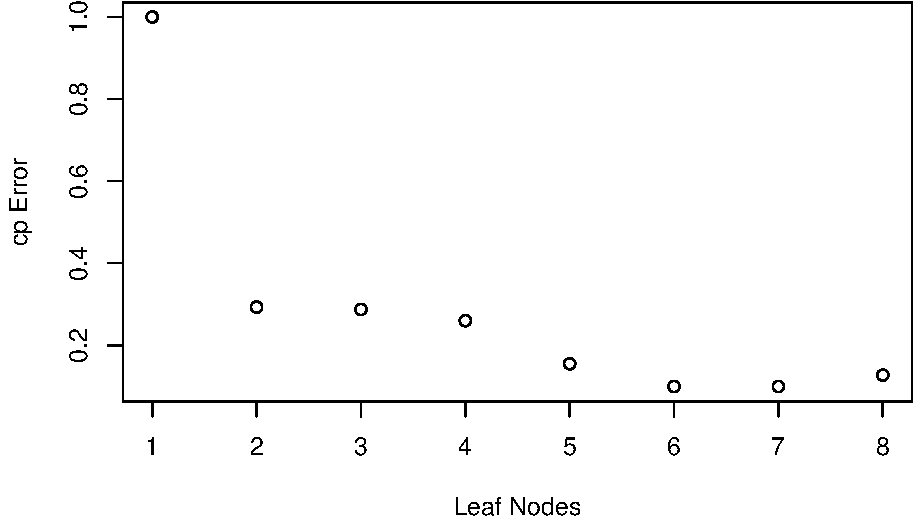
\includegraphics{HW4_Solution_files/figure-latex/unnamed-chunk-12-1.pdf}

~

\begin{center}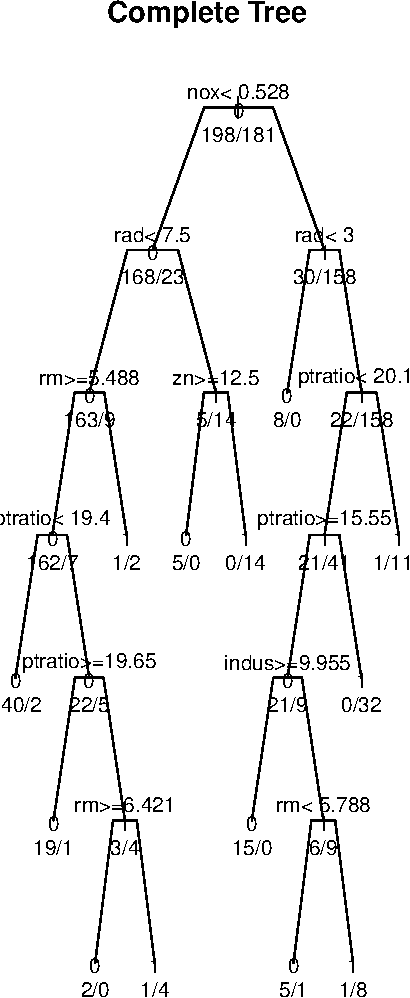
\includegraphics{HW4_Solution_files/figure-latex/unnamed-chunk-13-1} \end{center}

\begin{center}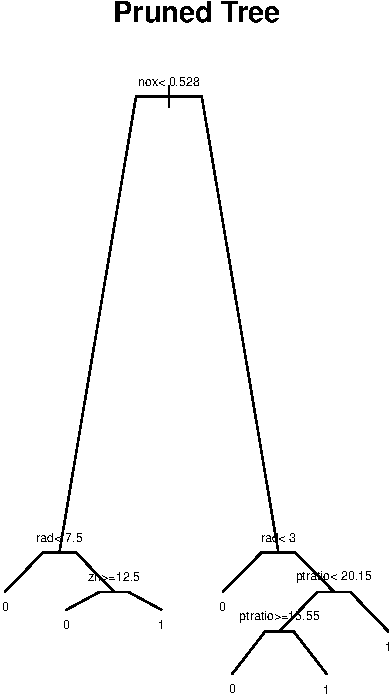
\includegraphics{HW4_Solution_files/figure-latex/unnamed-chunk-14-1} \end{center}

~

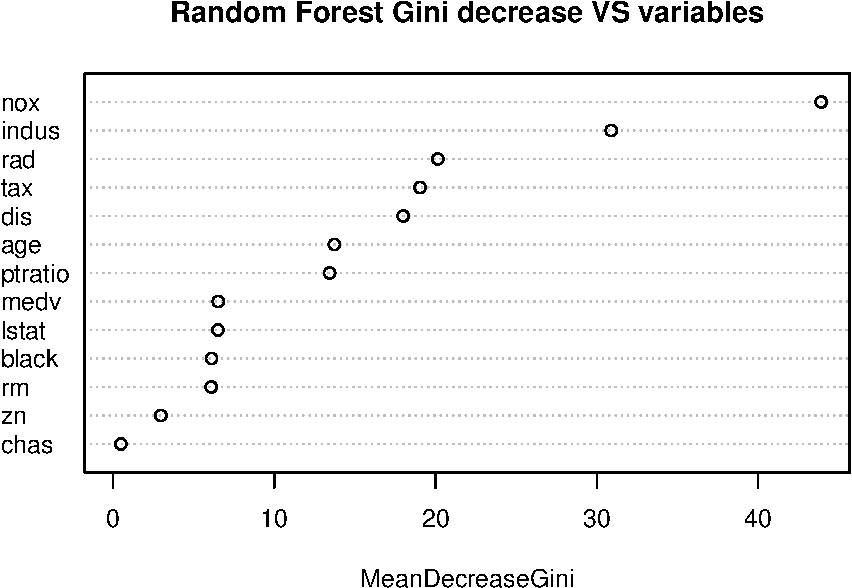
\includegraphics{HW4_Solution_files/figure-latex/unnamed-chunk-15-1.pdf}

\begin{verbatim}
##         MeanDecreaseGini
## zn             2.9634876
## indus         30.8929258
## chas           0.4865255
## nox           43.9133194
## rm             6.0905434
## age           13.7250842
## dis           17.9925855
## rad           20.1425671
## tax           19.0370443
## ptratio       13.4289716
## black          6.1108055
## lstat          6.5037884
## medv           6.5206467
\end{verbatim}

\begin{verbatim}
## Classification error for test error using Random Forest :  0.02362205
\end{verbatim}

~

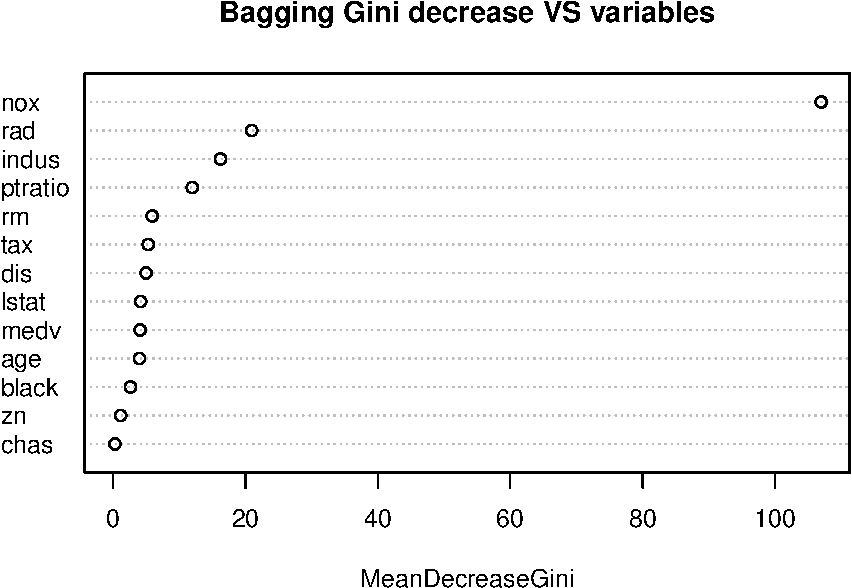
\includegraphics{HW4_Solution_files/figure-latex/unnamed-chunk-16-1.pdf}

\begin{verbatim}
##         MeanDecreaseGini
## zn             1.1537401
## indus         16.2273007
## chas           0.2892555
## nox          106.9821833
## rm             5.9202510
## age            3.9902632
## dis            4.9918628
## rad           20.9560436
## tax            5.3146915
## ptratio       11.9618871
## black          2.6293943
## lstat          4.1748335
## medv           4.0898553
\end{verbatim}

\begin{verbatim}
## Classification error for test error using Bagging : 0.01574803
\end{verbatim}

\begin{verbatim}
## Misclassification error for AdaBoost with shrinkage = 0.1 0.05189309
\end{verbatim}

\begin{verbatim}
## Misclassification error for AdaBoost with shrinkage = 0.6 0.04338883
\end{verbatim}

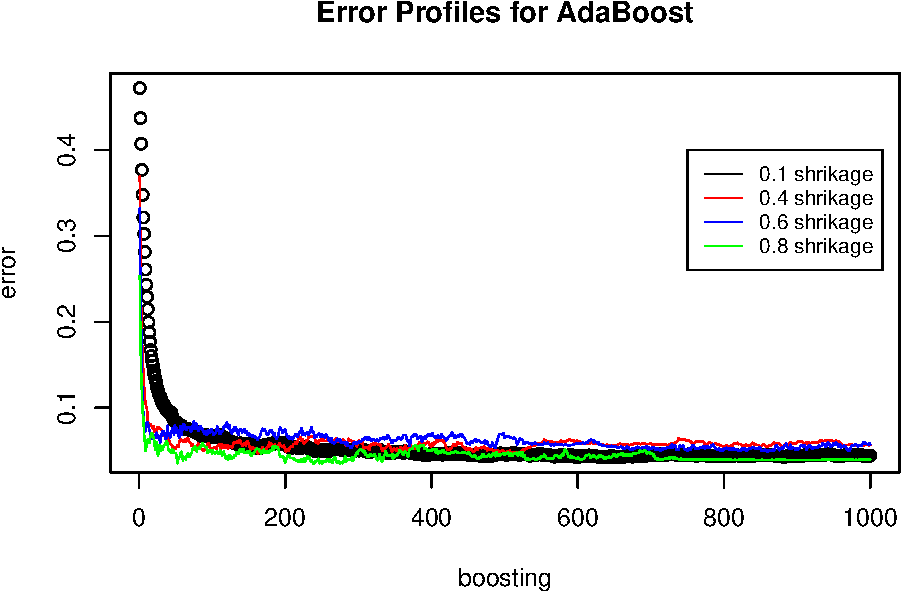
\includegraphics{HW4_Solution_files/figure-latex/unnamed-chunk-17-1.pdf}

We have implemented several methods for the Boston dataset such as
Random Forest, Bagging, Boosting(AdaBoost) and other simplistic methods
such as Logistic Regression and KNN. The errors on test sets were:
Logistic Regression = 0.1102, KNN = 0.0787, Random Forest = 0.0236,
Bagging = 0.1574, AdaBoost = 0.04338. From the Assignment 1 correlation
plot for the same dataset we saw that the variables were linearly
inseperable and hence we see a poor classification error by logistic
regression while the committee machines methods performs quite better
than logistic regression. We see that Bagging performs the best with a
test error of 0.01574. Also, KNN does not perform as good as the
committee machines methods because of high dimensional nature of our
data.

The only disadvantage of committee machines over the simple
classification methods for our data set is that it is computationally
expensive.


\end{document}
